\section{Плоское движение твёрдого тела. Преобразование координат}

\begin{definition}
  Движение, при котором все точки твёрдого тела, расположенные в плоскостях,
  параллельных некоторой неподвижной плоскости, во всё время движения остаются в
  тех же плоскостях, называется \textit{плоским движением}.

  Если разбить мысленно тело на плоские сечения, параллельные заданной
  плоскости, то эти сечения будут оставаться каждое в своей плоскости.
\end{definition}

\begin{figure}[H]
  \centering
  \resizebox{\linewidth}{!}{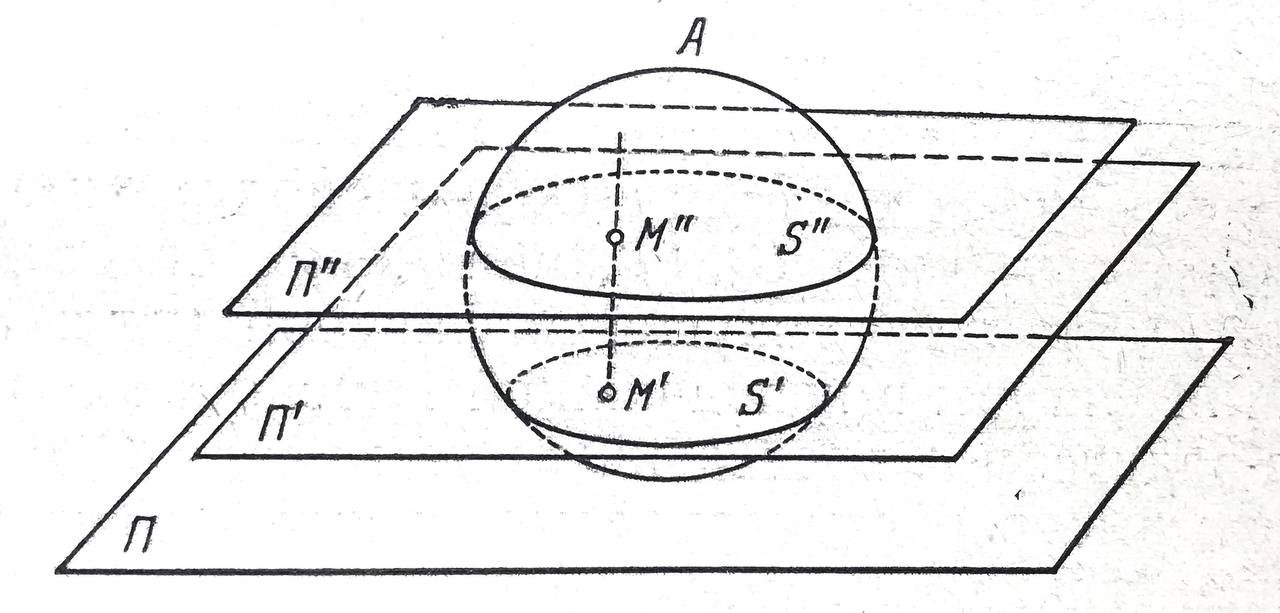
\includegraphics{src/mechanics/pictures/14_1.jpg}}

  \caption{}
  \label{fig:14_1}
\end{figure}

Пусть тело $A$ совершает действие, параллельное плоскости $\Pi$. Проведём
мысленно в теле ряд плоскостей $\Pi', \Pi'', \dots$, параллельных $\Pi$. Тело
разобьётся на ряд плоских фигур $S', S'', \dots$. Все точки, принадлежащие
какой-нибудь фигуре, движутся в плоскости фигуры, и, следовательно, фигура в
целом движется в своей плоскости. Движение одной такой плоской фигуры вполне
определяет движение всего твёрдого тела, так как плоскости, которыми мы разбили
твёрдое тело, друг с другом неизменно связаны и не могут двигаться друг по
отношению к другу.

Если мы возьмём в какой-нибудь фигуре $S'$ точку $M'$ и восставим в ней
перпендикуляр к плоскости фигуры $S'$, то точки $M'$ и $M''$ фигур $S'$ и $S''$,
лежащие на этом перпендикуляре, будут иметь одинаковое движение, то есть будут
описывать одинаковые траектории, иметь одинаковые скорости, одинаковые
ускорения.

Таким образом, можно значительно упростить изучение плоского движения твёрдого
тела --- достаточно изучить движение одной плоской фигуры в её плоскости.

\begin{figure}[H]
  \centering
  \resizebox{\linewidth}{!}{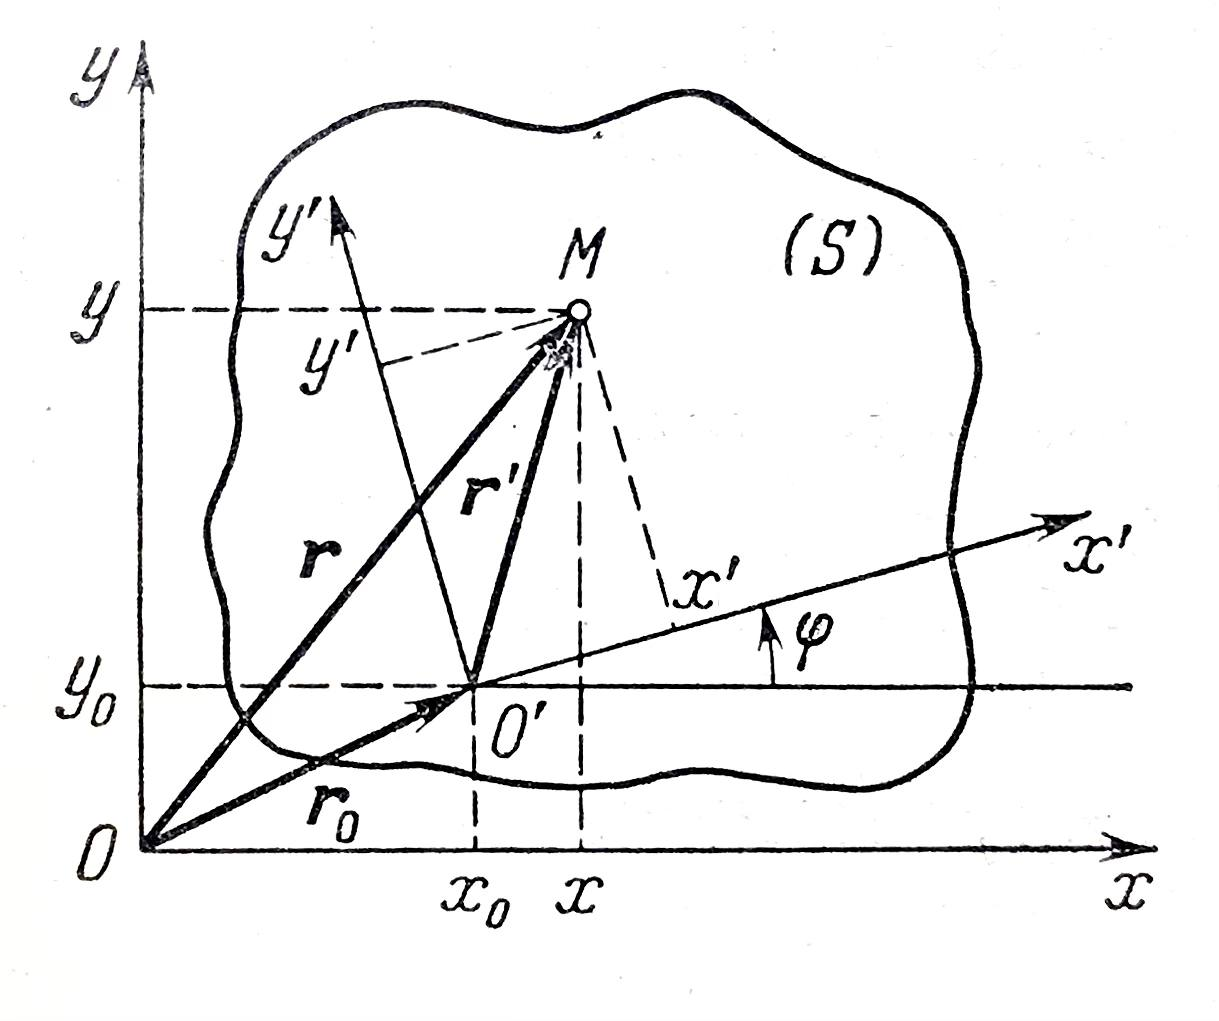
\includegraphics{src/mechanics/pictures/14_2.jpg}}

  \caption{}
  \label{fig:14_2}
\end{figure}

Возьмём две системы осей в плоскости движения фигуры: одну систему $Oxy$ ---
неподвижную, другую --- $O'x'y'$, неизменно связанную с движущейся фигурой.
Положение точки $M$ фигуры в неподвижной плоскости будем определять
вектор-радиусом $\vec{r}$, проведённым из начала $O$ неподвижной системы осей;
выбор рассматриваемой точки фигуры определяется указанием вектора $\pvec{r}$,
проведённого из начала $O'$ подвижной системы. Вектор-радиус начала $O'$
относительно $O$ обозначим через $\vec{r}_0$. Проекциями вектора $\vec{r}$ на
оси $x$ и $y$ будут декартовы координаты $x$ и $y$ в неподвижной системе осей;
при движении фигуры координаты $x$ и $y$ изменяются со временем; в
противоположность этому проекции вектора $\pvec{r}$ на подвижные оси, то есть
декартовы координаты $x'$ и $y'$ точки $M$ в системе подвижных осей, остаются
постоянными, как расстояния точек твёрдой фигуры до проведённых на ней прямых.

Всякой точке фигуры соответствует определённая пара чисел $x'$ и $y'$. В
частности, точке $O'$, началу подвижной системы, соответствуют значения $x'$ и
$y'$, равные нулю; значения координат $x$ и $y$ для этой точки обозначим через
$x_0$ и $y_0$ (проекции вектора $\vec{r}_0$).

Чтобы определить положение повдижной системы осей относительно неподвижной,
достаточно задать:
\begin{enumerate}
  \item положение начала $O'$, то есть вектор-радиус $\vec{r}_0$;
  \item угол одной из подвижных осей с одной из неподвижных, например угол
    $\varphi$ оси $x$ с осью $x'$.
\end{enumerate}
% TODO
(\textcolor{red}{TODO:} последнее требует некоторого уточнения)

\begin{definition}
  Начало $O'$ подвижной системы называется \textit{полюсом}; угол $\varphi$ будет в
  таком случае \textit{углом поворота} вокруг полюса.
\end{definition}

Плоское движение твёрдого тела определяется:
\begin{enumerate}
  \item уравнениями движения полюса
    \begin{equation}
      x_0 = f_1(t), \quad y_0 = f_2(t);
    \end{equation}
  \item уравнением вращения фигуры вокруг полюса
    \begin{equation}
      \varphi = \varphi(t).
    \end{equation}
\end{enumerate}

Чтобы получить уравнения движения любой точки плоской фигуры, спроектируем на
неподвижные оси $x$ и $y$ очевидное геометрическое равенство
\begin{equation*}
  \vec{r} = \vec{r}_0 + \pvec{r}.
\end{equation*}
Получим
\begin{equation}
  \label{eq:flat_point_motion}
  \begin{gathered}
    x = x_0 + x' \cos\varphi - y' \sin\varphi, \\
    y = y_0 + y' \sin\varphi + y' \cos\varphi.
  \end{gathered}
\end{equation}

Уравнения \ref{eq:flat_point_motion} представляют собой уравнения движения точки
$M$ или, что то же самое, параметрические уравнения её траектории.

\subsection{Список литературы}
\begin{enumerate}
  \item \cite{lourie}
\end{enumerate}

